\chapter{開発結果}

本章では,波の干渉と回折現象をプログラムによって視覚化した実行結果を記述する.

本研究では以下に挙げる物理現象の視覚化プログラムに取り組んだ.
\begin{enumerate}
\item 重ね合わせの原理を適用した波の干渉.
\item 波の回折現象.
\item 反射の法則.
\item 屈折の法則.
\end{enumerate}
これらのうち,1と2の現象は目標通りに視覚化することに成功したが, 3と4の法則の視覚化については未完成の部分を残す形となった. 3と4の未完成部分の考察については\ref{seq:considaration}章に記す.


\section{波の干渉の視覚化}
図\ref{fig:4wave}は指定した複数の点源から生成される円形波の位相変位をシミュレーションし,視覚化を行うプログラムである.
このプログラムにはdrawモードとcheckモードという2つのモードが実装されており,drawモードからcheckモードに移行するにはCキー(checkの頭文字).checkモードからdrawモードに移行するときはDキー(drawの頭文字)を押せばよい.


\begin{figure}[H]
 \begin{center}
  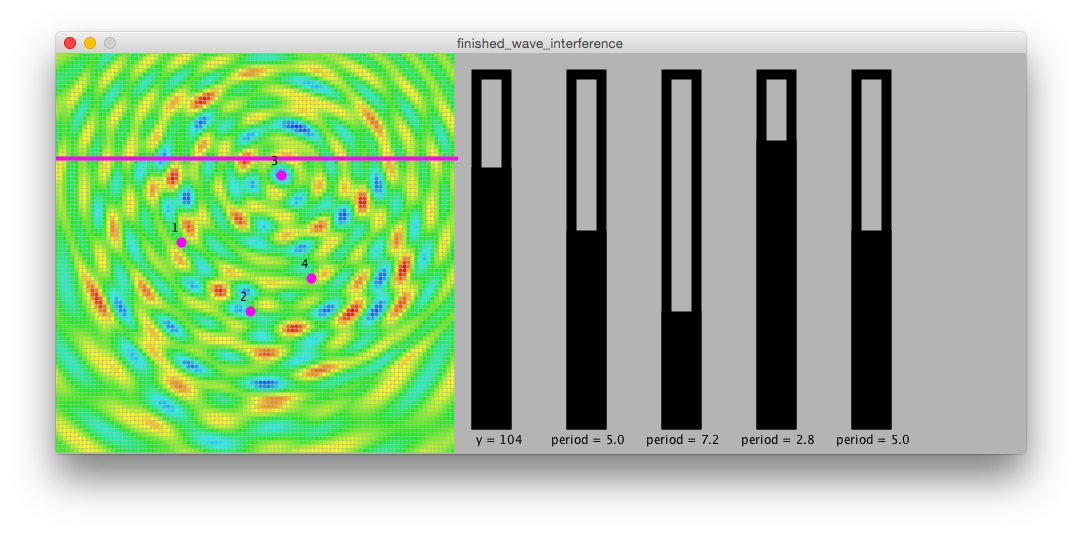
\includegraphics[width=\linewidth]{../result/4wave.png}
 \end{center}
 \caption{波の位相変位を視覚化したプログラムの画面.}
 \label{fig:4wave}
\end{figure}






\subsection{drawモード}
このモードは波源から生じる円形波を描写するモードである. プログラム起動時の画面が図\ref{fig:0wave}である.
画面左側の黒い領域が波を描写する領域,画面右側にはcheckモードで確認するy座標の位置を操作できるスライダーが配置されている. 
図\ref{fig:0wave}の状態で黒い領域上のいずれかの場所をクリックすると,クリックされた座標に波源が生成される.波源が生成されたあと,画面右側にはその波源の周期を変更できるスライダーが生成される.
\begin{figure}[H]
 \begin{center}
  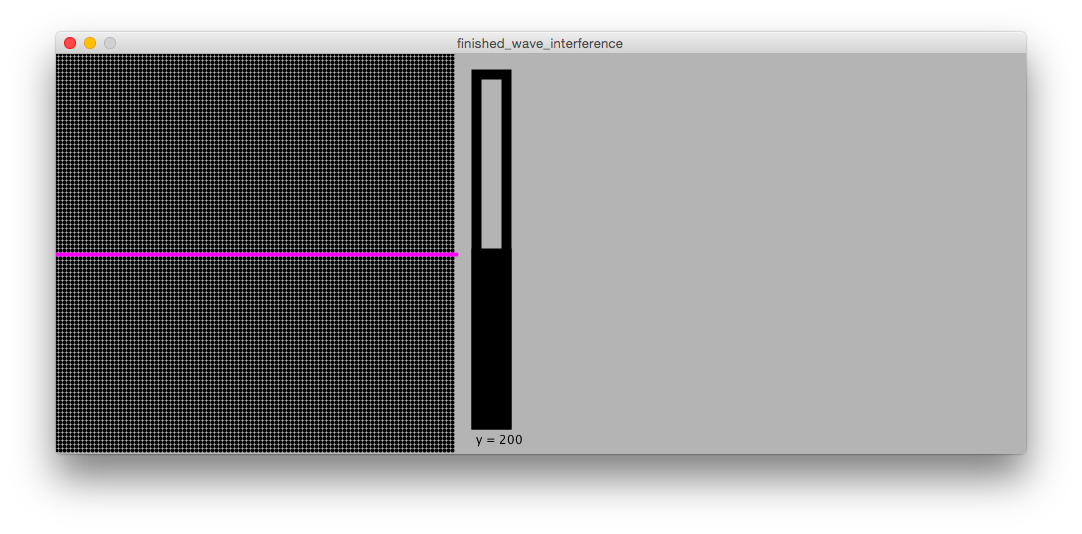
\includegraphics[width=110mm]{../result/0wave.png}
 \end{center}
 \caption{プログラム起動時の画面.}
 \label{fig:0wave}
\end{figure}



図\ref{fig:wave}は1つの波源を生成した後,周期をスライダーによって変更した様子である.
\begin{figure}[H]
 \begin{center}
  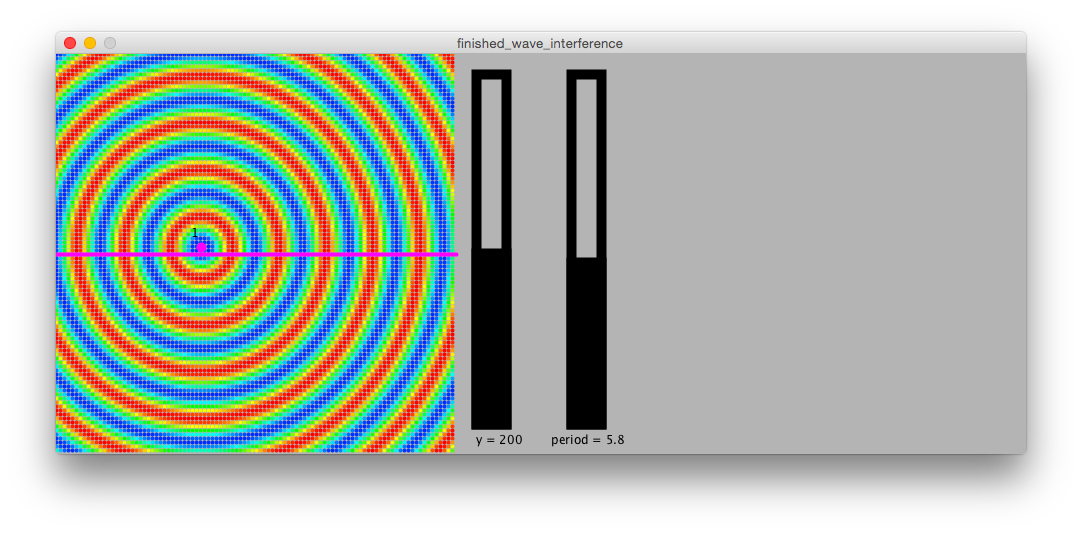
\includegraphics[width=110mm]{../result/wave.png}
 \end{center}
 \caption{1つの波の周期をスライダーで変更した画面.}
 \label{fig:wave}
\end{figure}
スライダーが周期を変更できる状態で
Lキー(lambdaの頭文字)を押すと,図\ref{fig:wavechangelambda}のように波の波長を変更できるスライダーに変化する.周期を変更するスライダーに戻したい場合はPキー(periodの頭文字)を押せばよい.

\begin{figure}[H]
 \begin{center}
  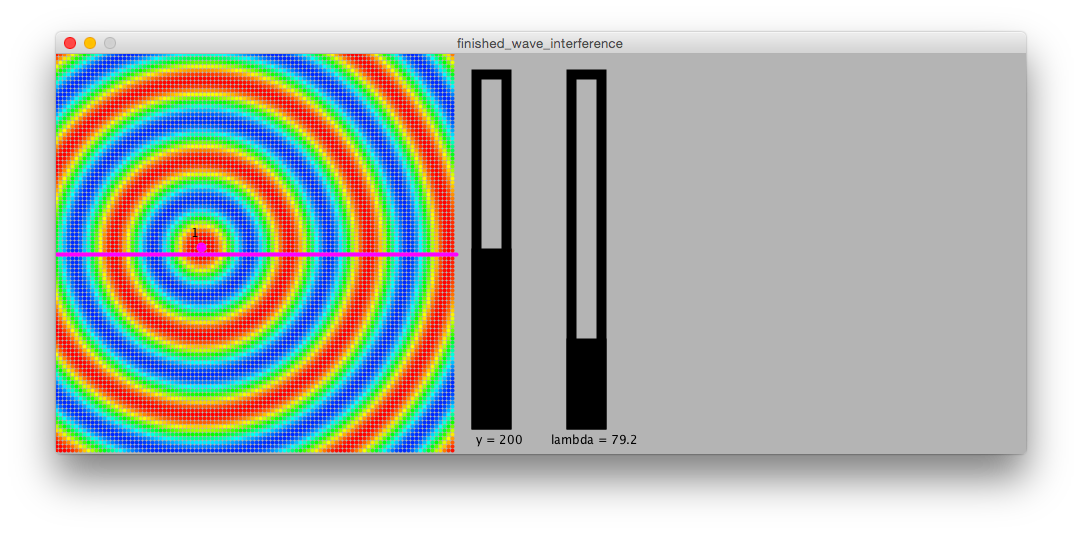
\includegraphics[width=110mm]{../result/wavechangelambda.png}
 \end{center}
 \caption{波長を変更できるスライダーに変化させた時の画面.}
 \label{fig:wavechangelambda}
\end{figure}
\newpage
波源は図\ref{fig:5wave}のように5個まで生成できる.
\begin{figure}[htbp]
 \begin{center}
  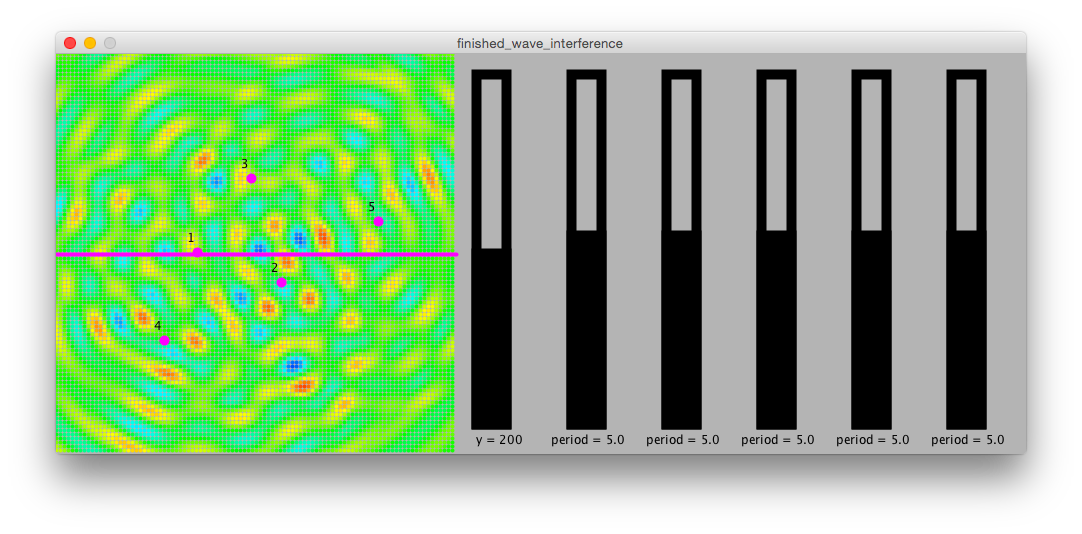
\includegraphics[width=\linewidth]{../result/5wave.png}
 \end{center}
 \caption{波源を5個生成した時の画面.}
 \label{fig:5wave}
\end{figure}
\subsection{checkモード}
\label{sec:check}
このモードはdrawモードに描写されている赤い線上の変位をリアルタイムに視覚化するモードである.同時刻,同座標で周期,波長が同一な波を生成し,波を生成して360フレーム目の状態をdrawモード,checkモードでそれぞれ描写したのが図\ref{fig:compare}(\subref{drawmode}),(\subref{checkmode})である.


\begin{figure}[H]
\begin{minipage}[b]{1.0\linewidth}
\centering
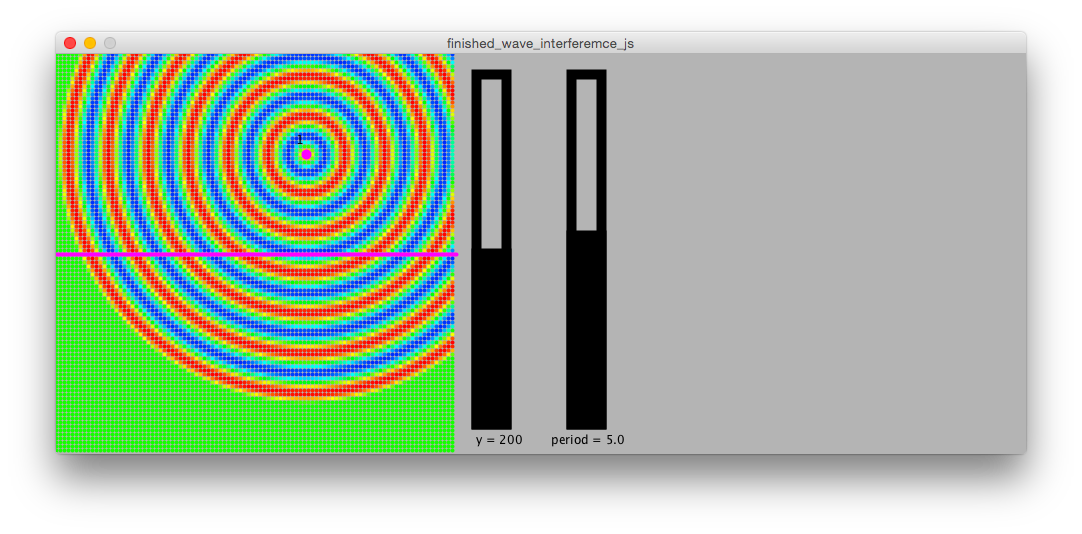
\includegraphics[keepaspectratio, scale=0.40]
  {../result/drawmode.png}
 \subcaption{drawモード.}\label{drawmode}
 \end{minipage}
 
\begin{minipage}[b]{1.0\linewidth}
\centering
  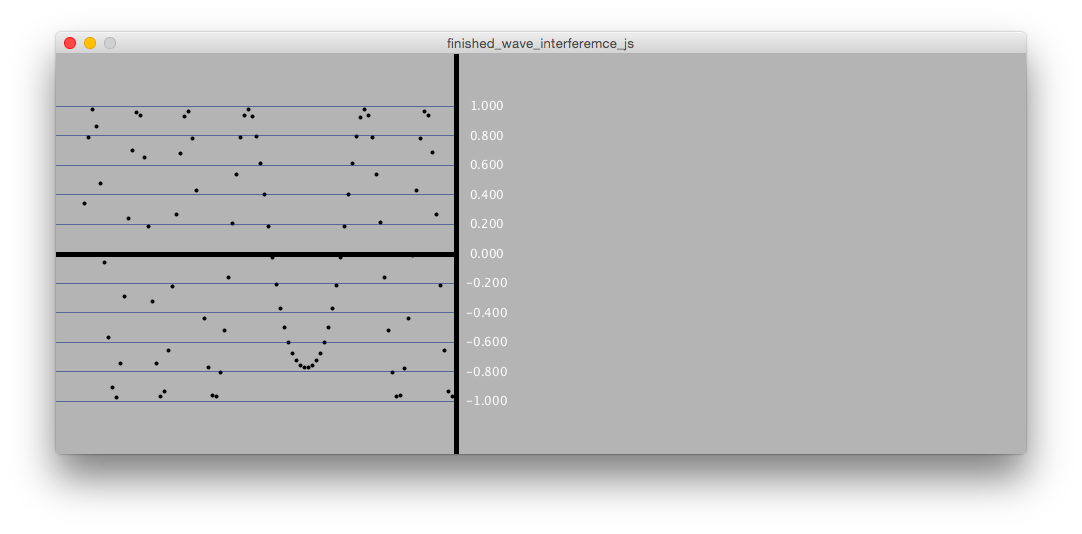
\includegraphics[keepaspectratio, scale=0.40]
  {../result/checkmode.png}
 \subcaption{checkモード.}\label{checkmode}
 \end{minipage}
  
  \caption{周期5.0,波長40.0の波が生成されてから360フレーム目のdrawモード,checkモード.}
 \label{fig:compare}
\end{figure}
\section{波の回折現象の視覚化}
\label{defraction}
図\ref{fig:diffractiondemo}は障害物の間に一定の間隔で配置された波源から生成される円形波によって,波の回折現象の視覚化を行うプログラムである.

\begin{figure}[H]
 \begin{center}
  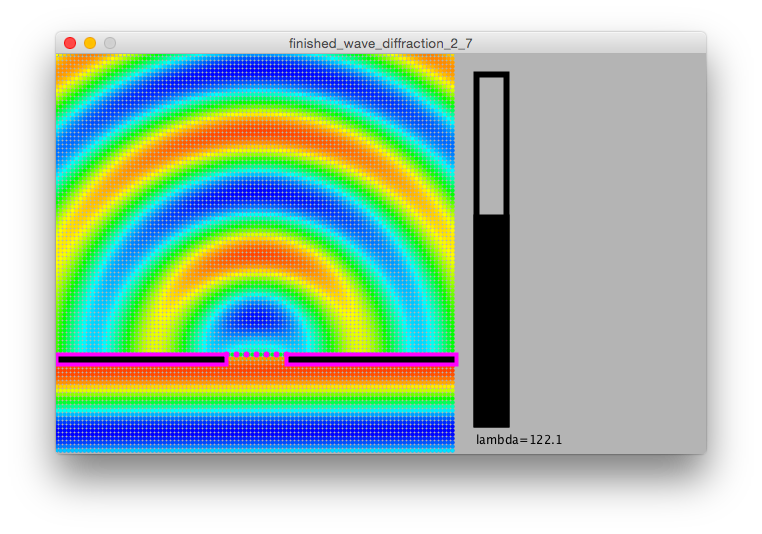
\includegraphics[width=120mm]{../result/diffractiondemo.png}
 \end{center}
 \caption{回折現象の視覚化.}
 \label{fig:diffractiondemo}
\end{figure}


プログラムを起動すると図\ref{fig:ds1}の画面になる.
この画面では画面右にあるスライダーで,障害物の隙間の間隔を調節できる.長さの値はスライダー下部に表示されており,図\ref{fig:ds2}のように長さの値に応じて波源の数が決定される.
\begin{figure}[H]
\begin{minipage}{0.5\hsize}
\begin{center}
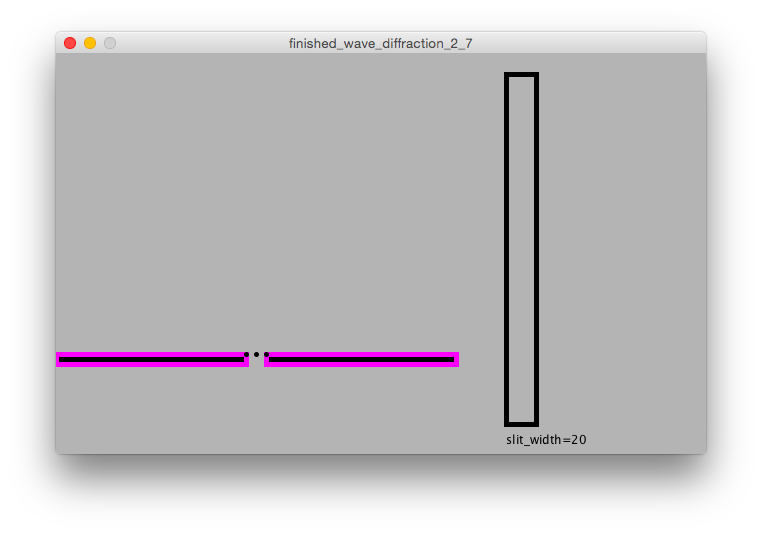
\includegraphics[width=\linewidth]
  {../result/diffractionstart1.png}
\caption{初期状態}
\label{fig:ds1}
\end{center}
\end{minipage}%
\begin{minipage}{0.5\hsize}
\begin{center}
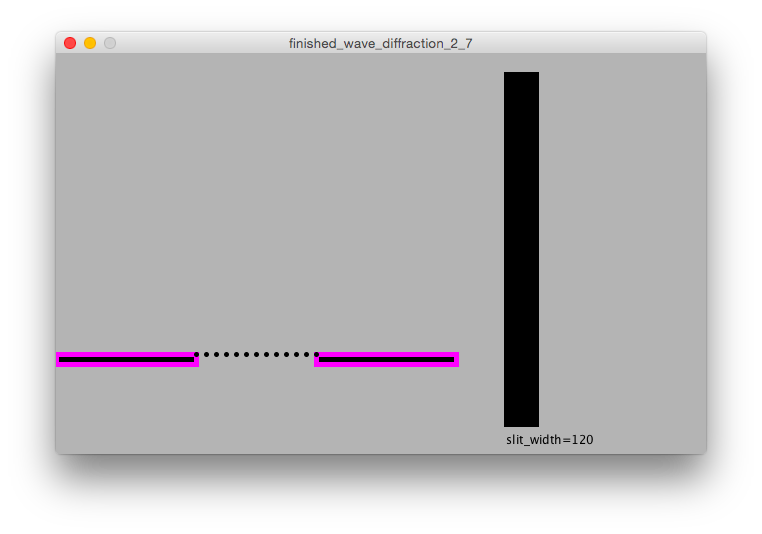
\includegraphics[width=\linewidth]
  {../result/diffractionstart2.png}
\caption{隙間の間隔を120に設定した様子}
\label{fig:ds2}
\end{center}
\end{minipage}
\end{figure}



これらの画面でSキー(Startの頭文字)を押すと,図\ref{fig:incident}の画面へと切り替わる.図\ref{fig:incident}の画面は画面下部から平行に進行してきた入射波が波源に到達すると,図\ref{fig:diffraction1}のように円形波が生成され,波長に応じた挙動を描写する.
\begin{figure}[H]
\begin{minipage}{0.5\hsize}
\begin{center}
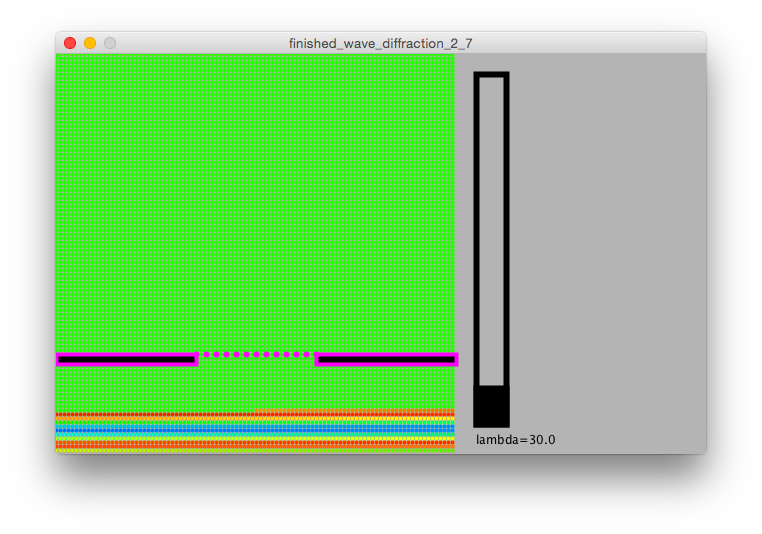
\includegraphics[width=\linewidth]
  {../result/diffraction1.png}
\caption{入射波の描写}
\label{fig:incident}
\end{center}
\end{minipage}%
\begin{minipage}{0.5\hsize}
\begin{center}
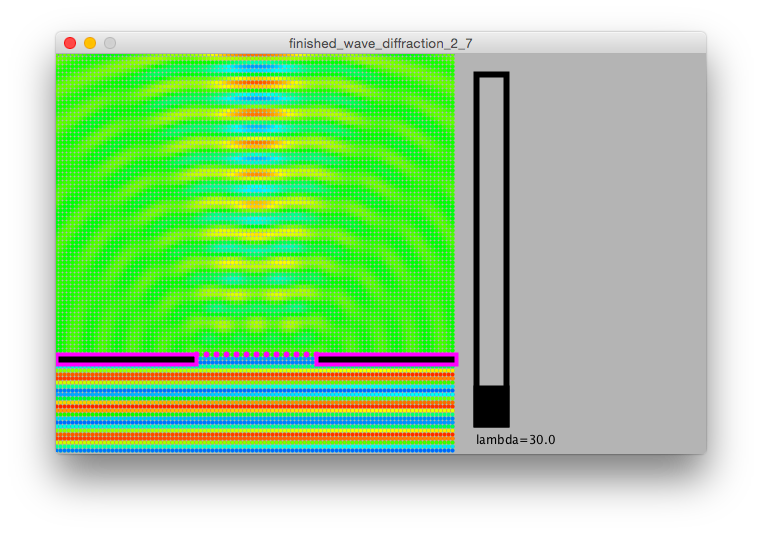
\includegraphics[width=\linewidth]
  {../result/diffraction2.png}
\caption{隙間の間隔=120,波長=30.0}
\label{fig:diffraction1}
\end{center}
\end{minipage}
\end{figure}


波長を変えると図\ref{fig:diffraction3}のように,図\ref{fig:diffraction3}と同じ波長の値のまま隙間の間隔を小さくしてシミュレーションすると図\ref{fig:diffraction4}のようになる.
\begin{figure}[H]
\begin{minipage}{0.5\hsize}
\begin{center}
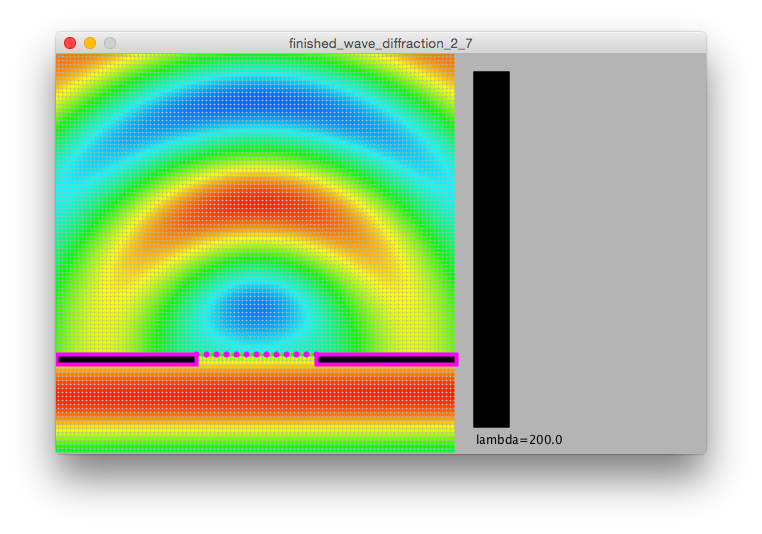
\includegraphics[width=\linewidth]
  {../result/diffraction3.png}
\caption{隙間の間隔=120,波長=200.0}
\label{fig:diffraction3}
\end{center}
\end{minipage}%
\begin{minipage}{0.5\hsize}
\begin{center}
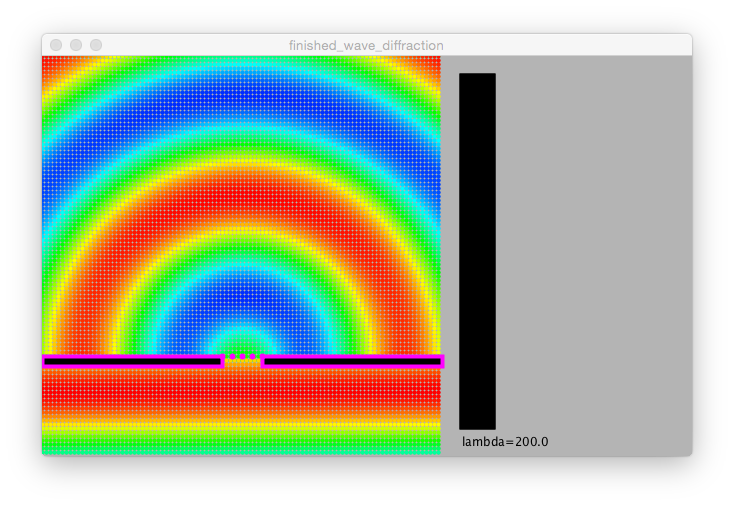
\includegraphics[width=\linewidth]
  {../result/diffraction4.png}
\caption{隙間の間隔=40,波長=200.0}
\label{fig:diffraction4}
\end{center}
\end{minipage}
\end{figure}

\begin{comment}
\section{反射の法則の視覚化}
\label{seq:reflection}
図\ref{fig:reflectionsetumei}は反射面に一定の間隔で配置された波源から生成される円形波の位相情報から反射角を描写するプログラムである.
\begin{figure}[H]
 \begin{center}
  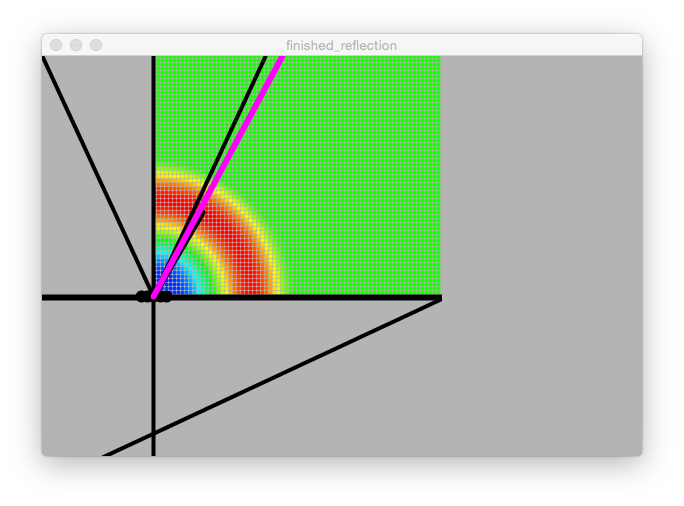
\includegraphics[width=110mm]{../result/reflectionsetumei.png}
 \end{center}
 \caption{プログラムの動作の様子.}
 \label{fig:reflectionsetumei}
\end{figure}

プログラムを起動すると図\ref{fig:reflectionincident}のように入射波となる平行波が画面左上から右下にかけて進んでくる.波源は入射波の速度に応じた間隔で5つ生成される.

入射角が20度の入射波によって各波源が生成され,それらから生じた波を描写したものが図\ref{fig:reflection20}である.図\ref{fig:reflection20}の画面右上の波の描写領域に注目すると3本の線がある.

画面の上端に届いていない黒線は,3個目の波源(入射角と反射角の境界線)から現在の最大変位を結んだものである.各フレームごとに最大変位が変わるため,この線もそれに応じて更新される.

赤線は各フレームごとの最大変位をとる座標の傾きを平均化して描写したものである.\ref{seq:pxcelproblem}節で詳しく取り扱うが,プログラムの仕様上,理論上の最大変位を取得することは出来ないので値を平均化することで精度を高める目的がある.

もう一つの黒線は,反射の法則を満たす角度で3個目の波源から引いた線である.この線と赤線のずれを無くすことを目標としていた.
\begin{figure}[H]
\begin{minipage}{0.5\hsize}
\begin{center}
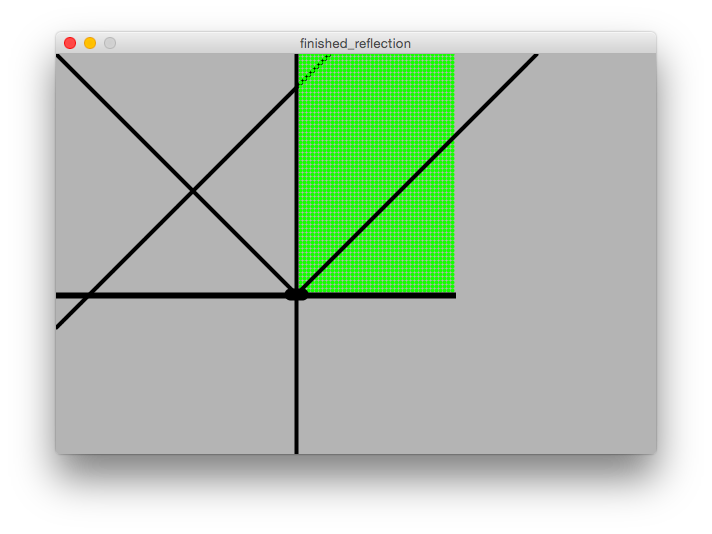
\includegraphics[width=\linewidth]
  {../result/reflectionincident.png}
\caption{入射波が進行する様子}
\label{fig:reflectionincident}
\end{center}
\end{minipage}%
\begin{minipage}{0.5\linewidth}
\begin{center}
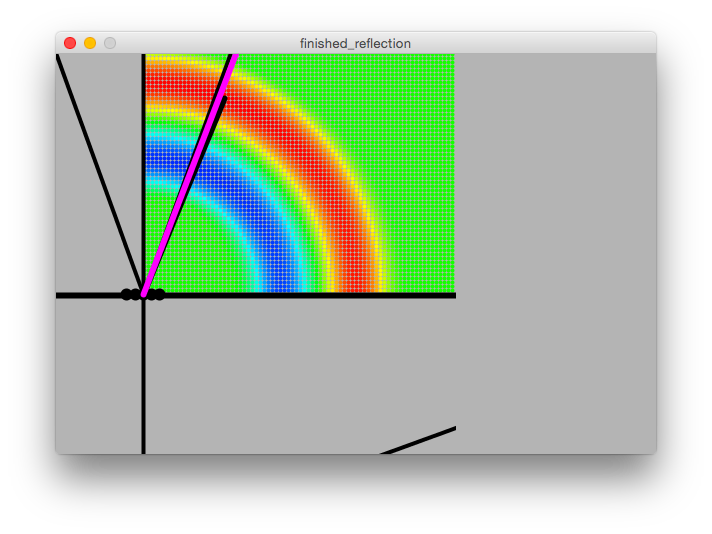
\includegraphics[width=\linewidth]
  {../result/reflectionangle20.png}
\caption{入射角を$20^{\circ}$に設定した波が進行する様子.}
\label{fig:reflection20}
\end{center}
\end{minipage}
\end{figure}

入射波を$20^{\circ}$に設定した結果が図\ref{fig:reflection20finish}, $40^{\circ}$に設定した結果が図\ref{fig:reflection40finish}である.
\begin{figure}[H]
\begin{minipage}{0.5\hsize}
\begin{center}
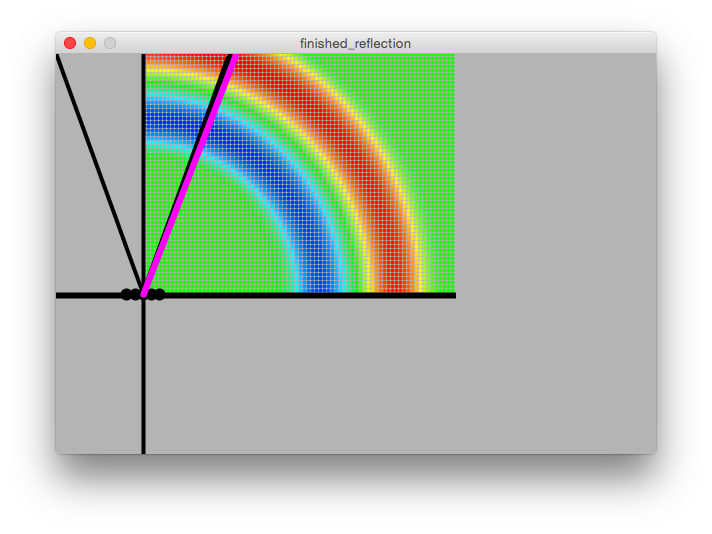
\includegraphics[width=\linewidth]
  {../result/finishreflectionangle20.png}
\caption{入射角が$20^{\circ}$の時の反射角の結果.}
\label{fig:reflection20finish}
\end{center}
\end{minipage}%
\begin{minipage}{0.5\linewidth}
\begin{center}
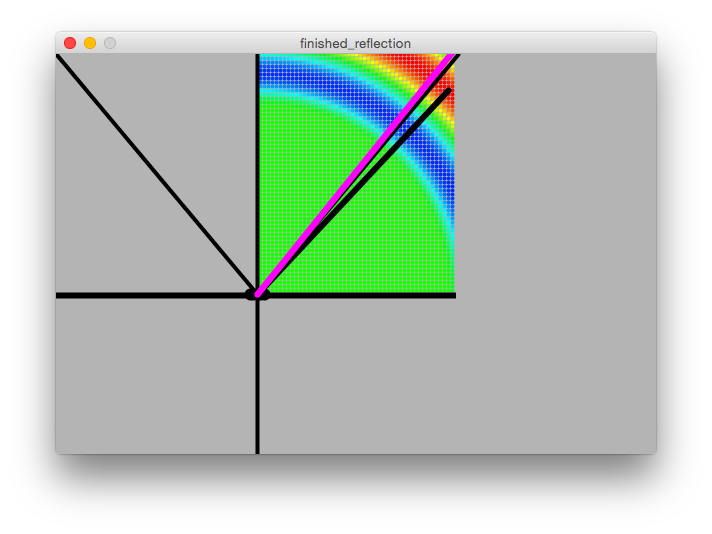
\includegraphics[width=\linewidth]
  {../result/finishreflectionangle40.png}
\caption{入射角が$40^{\circ}$の時の反射角の結果.}
\label{fig:reflection40finish}
\end{center}
\end{minipage}
\end{figure}

図\ref{fig:reflection20finish},図\ref{fig:reflection40finish}を見ると僅かながらずれが生じており,本研究ではこのずれを修正することが出来なかった.ずれが生じる原因,改善案については\ref{considaration}章で議論する.

\section{屈折の法則の視覚化}
図\ref{fig:refraction}は屈折率が1.5の媒質に,入射角$30^{\circ}$の入射波が進行した際の屈折角の角度を示すプログラムである.


\begin{figure}[H]
 \begin{center}
  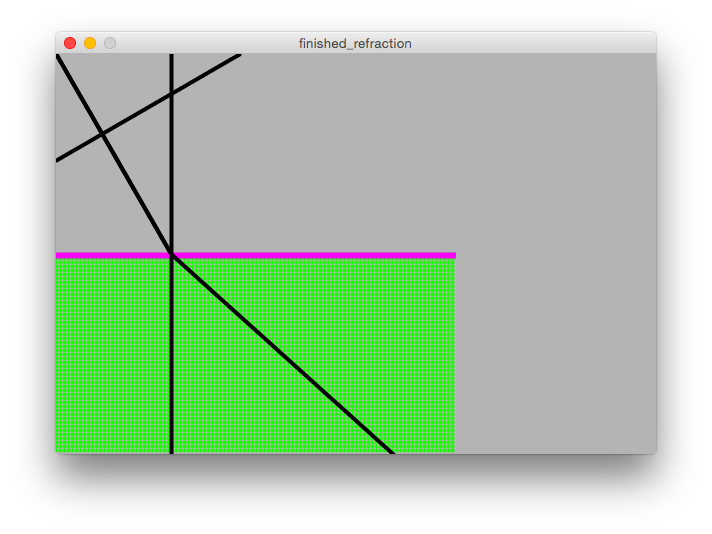
\includegraphics[width=130mm]{../result/refractionangle3015.png}
 \end{center}
 \caption{入射角に対する反射角の角度.}
 \label{fig:refraction}
\end{figure}

この後,媒質に応じた速度の素元波を発生させ,\ref{seq:reflection}節で用いた方法と同じ要領で屈折角を描写しようと考えていたが,反射角の描写が理論通りにできていないので,処理の実装に取り掛かることができなかった.
\end{comment}